\subsection{ソフトウェア要求の基礎}

\subsubsection{ソフトウェア要求の定義}

\term{ソフトウェア要求}とは、利用者が問題を解決したり目的を達成したりするために必要な条件または能力である。また、契約、標準、仕様、法令などを満たすために、システムや構成要素が備えるべき条件または能力でもある。さらに、それらを文書やモデルとして表したものも要求と呼ぶ。

より実務的に言えば、ソフトウェア要求とは「何を満たせば、現実世界の問題を解決したと言えるか」を表す合意である。ここでいう「問題」は、業務の自動化、既存ソフトウェアの欠点の修正、機器の制御、利用者体験の改善、規制への対応など、さまざまである。

\begin{definitionbox}ソフトウェア要求とは、ソフトウェアまたはソフトウェアを作るプロジェクトが満たすべき条件・能力・制約を、関係者が共有できるように表したものである。\end{definitionbox}

要求は通常、顧客、利用者、業務担当者から出る。しかし、それだけではない。規制当局、標準、既存システム、運用部門、サポート部門、開発組織、プロジェクト計画そのものも要求の源泉になる。

\subsubsection{ソフトウェア要求の分類}

要求は、すべてをひとまとめにすると扱いにくい。SWEBOKでは、ソフトウェア要求を大きく次のように整理する。

\begin{center}
\footnotesize
\par\smallskip\noindent\refstepcounter{table}\label{tab:ch01-02}\textbf{表 \thetable: 第01章 ソフトウェア要求 表02}\par\smallskip
\begin{tabular}{c}
ソフトウェア要求 \\
$\downarrow$ \\
ソフトウェア製品要求 \quad / \quad ソフトウェアプロジェクト要求 \\
$\downarrow$ \\
機能要求 \quad / \quad 非機能要求 \\
$\downarrow$ \\
技術制約 \quad / \quad サービス品質制約
\end{tabular}
\end{center}

\begin{figure}[htbp]
\centering
\IfFileExists{assets/generated_figures/ch01/fig-ch01-02.png}{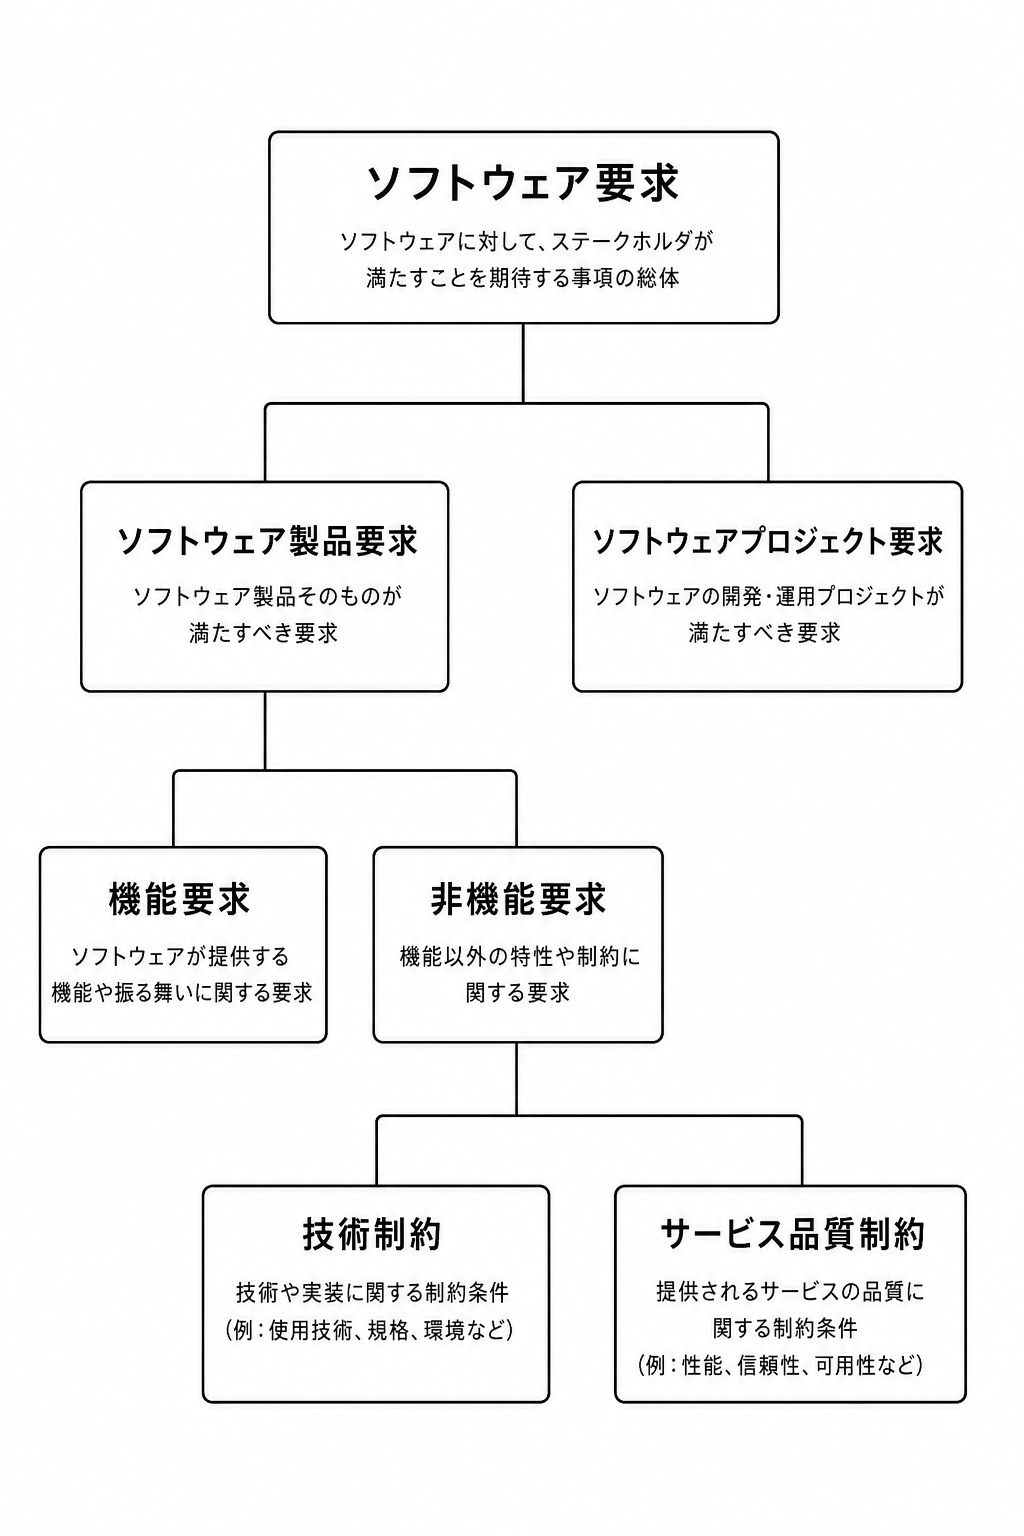
\includegraphics[width=0.96\linewidth]{assets/generated_figures/ch01/fig-ch01-02.png}}{\fbox{\parbox[c][48mm][c]{0.9\linewidth}{\centering 画像生成待ち\\要求分類の階層図}}}
\caption{要求分類の階層図}
\label{fig:ch01-02}
\end{figure}

分類の目的は、単に用語を覚えることではない。分類すると、要求の源泉、引き出し方、分析方法、仕様化の方法、確認すべき相手が見えやすくなる。

\subsubsection{ソフトウェア製品要求とソフトウェアプロジェクト要求}

\term{ソフトウェア製品要求}は、完成するソフトウェアそのものが満たすべき性質である。画面、処理、データ、外部連携、性能、信頼性、セキュリティなどが含まれる。

\term{ソフトウェアプロジェクト要求}は、ソフトウェアを作るプロジェクトの進め方を制約する要求である。費用、納期、人員、テスト環境、データ移行、利用者教育、保守準備などが例である。プロジェクト要求は、プロジェクト憲章、契約、計画書などに記録されることが多い。

\par\smallskip\noindent\refstepcounter{table}\label{tab:ch01-03}\textbf{表 \thetable: 第01章 ソフトウェア要求 表03}\par\smallskip
\begin{tabularx}{0.97\linewidth}{@{}p{.28\linewidth}X@{}}
\toprule
区分 & 見分け方 \\
\midrule
\term{製品要求} & 完成したソフトウェアがどう振る舞うか、どの品質を満たすかを述べる。 \\
\term{プロジェクト要求} & 開発の費用、納期、人員、進め方、移行、教育などを縛る。 \\
\bottomrule
\end{tabularx}

\MiniBox{例}{「利用者は注文履歴を検索できる」は製品要求である。「本番移行は年度末までに完了する」はプロジェクト要求である。}

\subsubsection{機能要求}

\term{機能要求}とは、ソフトウェアが提供すべき観測可能な振る舞いを表す要求である。言い換えると、「ソフトウェアが何をするか」を述べる要求である。

機能要求は、二つの観点で理解しやすい。第一に、\term{方針}である。方針とは、常に守られるべき規則である。たとえば銀行システムでは、「口座は少なくとも一人の所有者を持つ」「口座残高は負にならない」といった要求が該当する。第二に、\term{プロセス}である。プロセスとは、実行される業務手続きである。入金、出金、振込、予約、取消、検索、承認などが該当する。

\begin{definitionbox}機能要求とは、ソフトウェアが実行すべき処理、守るべき業務規則、利用者に提供すべき振る舞いを述べる要求である。\end{definitionbox}

\subsubsection{非機能要求}

\term{非機能要求}とは、ソフトウェアの実装技術や運用品質を制約する要求である。「何をするか」ではなく、「どのような条件で、どの水準で、どの技術的制約のもとで実現するか」に関わる。

非機能要求には、性能、応答時間、信頼性、正確性、可用性、拡張性、保存容量、プラットフォーム、利用するデータベースなどが含まれる。非機能要求はさらに、\term{技術制約}と\term{サービス品質制約}に分けると理解しやすい。

\MiniBox{注意}{「非機能要求」は「重要でない要求」という意味ではない。むしろ、性能、信頼性、セキュリティ、安全性など、失敗したときの影響が大きい要求が多い。}

\subsubsection{技術制約}

\term{技術制約}とは、特定の自動化技術やインフラを使うこと、または使わないことを指定する要求である。ここでは「名前のある技術を指定しているか」に注目すると見分けやすい。

\par\smallskip\noindent\refstepcounter{table}\label{tab:ch01-04}\textbf{表 \thetable: 第01章 ソフトウェア要求 表04}\par\smallskip
\begin{tabularx}{0.97\linewidth}{@{}p{.25\linewidth}X@{}}
\toprule
対象 & 例 \\
\midrule
プラットフォーム & Windows、macOS、Android、iOS など。 \\
プログラミング言語 & Java、C++、C\#、Python など。 \\
ブラウザ & Chrome、Safari、Edge など。 \\
データベース & Oracle、SQL Server、MySQL など。 \\
禁止事項 & ポインタ利用禁止、特定暗号方式の禁止、外部クラウド利用禁止など。 \\
\bottomrule
\end{tabularx}

技術制約は、既存システムとの連携、組織標準、保守要員のスキル、セキュリティ方針、ライセンス方針などから生じることが多い。

\subsubsection{サービス品質制約}

\term{サービス品質制約}とは、特定の技術名を指定せず、ソフトウェアが達成すべき品質水準を表す要求である。サービス品質という表現は、利用者や運用者が受け取るサービスの品質として考えるとわかりやすい。

\par\smallskip\noindent\refstepcounter{table}\label{tab:ch01-05}\textbf{表 \thetable: 第01章 ソフトウェア要求 表05}\par\smallskip
\begin{tabularx}{0.97\linewidth}{@{}p{.26\linewidth}X@{}}
\toprule
品質水準 & 要求文の例 \\
\midrule
応答時間 & 通常時、検索結果を2秒以内に返す。 \\
スループット & 1分あたり1万件のイベントを処理する。 \\
正確性 & 金額計算は定められた丸め規則に従う。 \\
信頼性 & 月間稼働率99.9\%以上を維持する。 \\
拡張性 & 利用者数が10倍になっても構成変更で対応できる。 \\
セキュリティ & 権限のない利用者は個人情報を閲覧できない。 \\
\bottomrule
\end{tabularx}

\subsubsection{なぜこのように分類するのか}

要求を分類する理由は、実務上は非常に明確である。

\begin{itemize}
\item 要求の種類によって、要求の源泉が異なる。
\item 源泉が異なれば、聞き出し方も異なる。
\item 種類によって、分析方法、仕様化方法、確認すべき相手が異なる。
\item 要求の種類によって、設計・実装・テストへの影響が異なる。
\end{itemize}

さらに、分類は複雑さを下げる。業務規則を議論している最中に、同時にデータベース製品や処理速度を議論すると、論点が混ざる。機能要求、技術制約、サービス品質制約を分ければ、業務の専門家は業務の観点に集中でき、技術者は技術の観点に集中できる。

\MiniBox{完全技術フィルタ}{機能要求と非機能要求の境界が曖昧なときは、「無限に速く、記憶容量が無限で、費用がゼロで、故障しない理想的なコンピュータがあっても、その要求を書く必要があるか」と問う。必要なら機能要求である。不要なら、技術や品質に関する制約、つまり非機能要求である。}

\begin{figure}[htbp]
\centering
\IfFileExists{assets/generated_figures/ch01/fig-ch01-03.png}{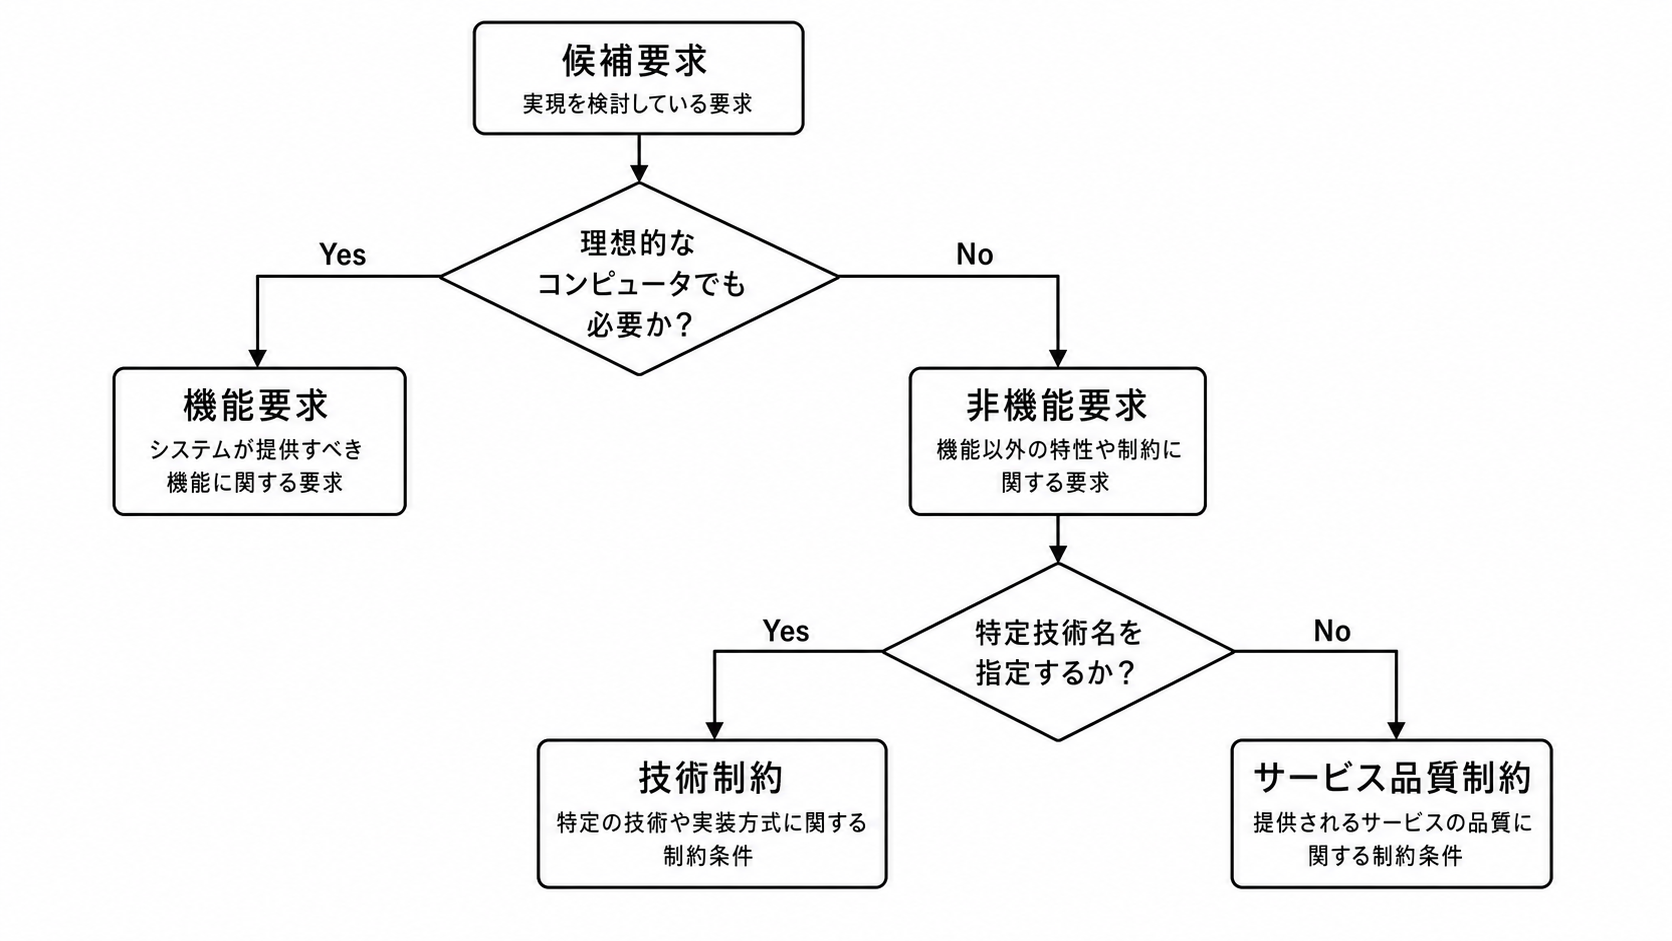
\includegraphics[width=0.96\linewidth]{assets/generated_figures/ch01/fig-ch01-03.png}}{\fbox{\parbox[c][48mm][c]{0.9\linewidth}{\centering 画像生成待ち\\完全技術フィルタの判定フロー}}}
\caption{完全技術フィルタの判定フロー}
\label{fig:ch01-03}
\end{figure}

\subsubsection{システム要求とソフトウェア要求}

\term{システム要求}は、ソフトウェアだけでなく、ハードウェア、ファームウェア、人、情報、手順、設備、サービス、支援要素を含むシステム全体に対する要求である。自動運転車、医療機器、工場制御、航空機システムのように、複数の要素が組み合わさる場合には、システム要求とソフトウェア要求を分けて扱うことが重要である。

\term{ソフトウェア要求}は、その大きなシステムの中で、ソフトウェア要素が満たすべき要求である。たとえば「車両は障害物を検知して安全に停止する」はシステム要求であり、その一部として「認識ソフトウェアは前方物体を一定時間内に分類する」といったソフトウェア要求が割り当てられる。

\begin{figure}[htbp]
\centering
\IfFileExists{assets/generated_figures/ch01/fig-ch01-04.png}{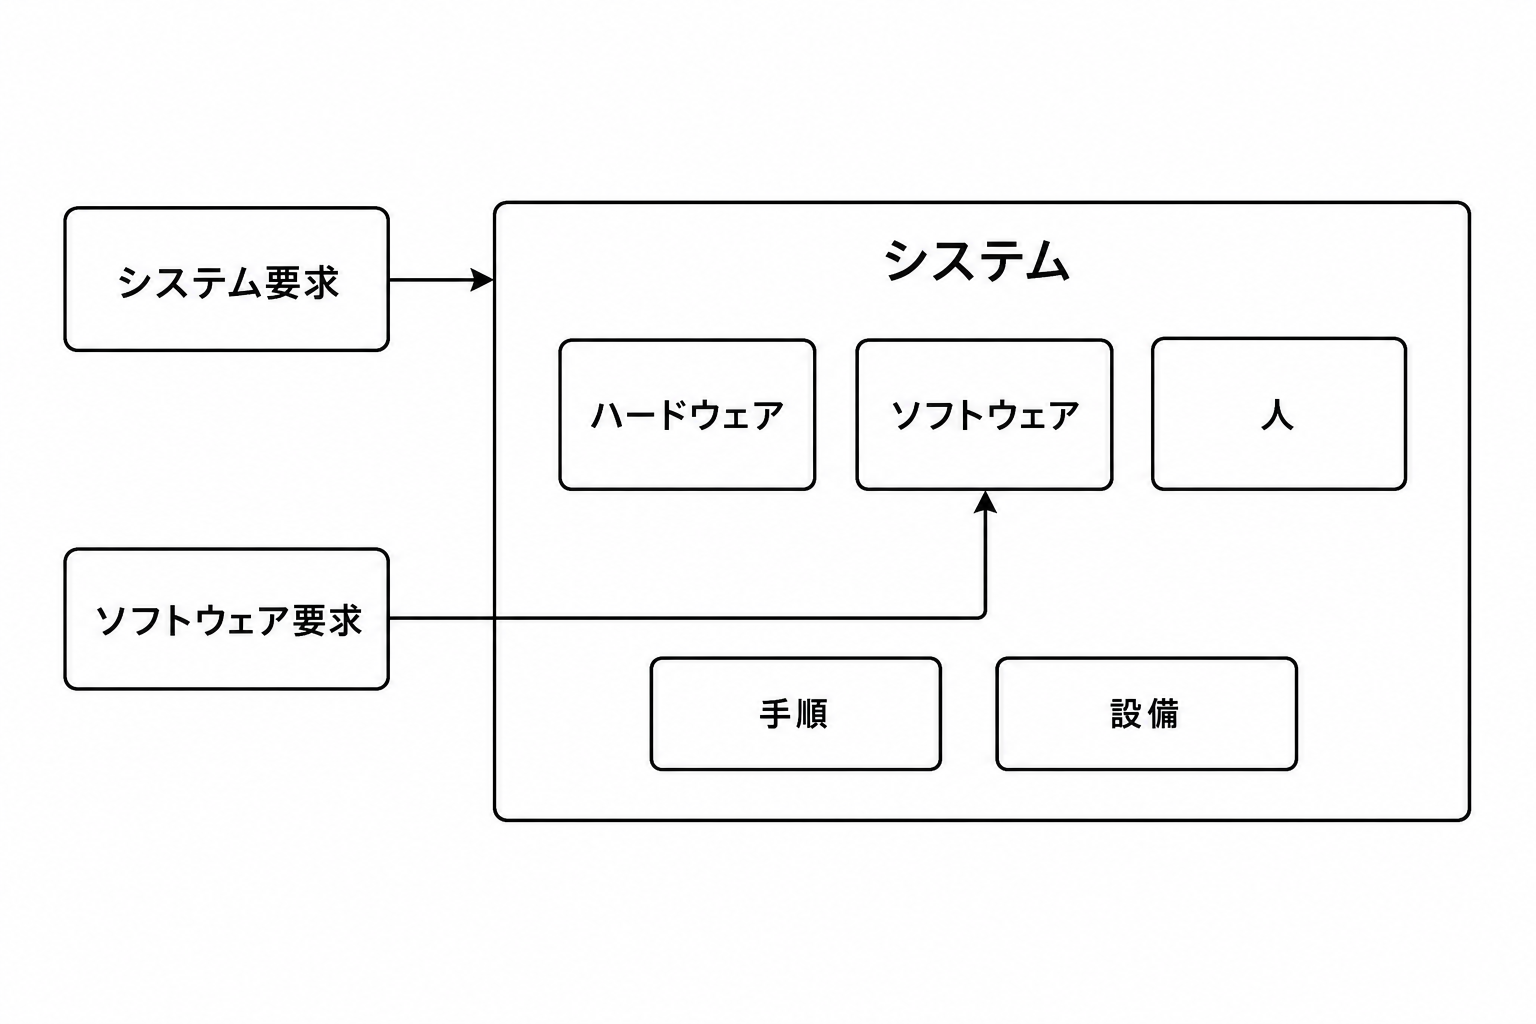
\includegraphics[width=0.96\linewidth]{assets/generated_figures/ch01/fig-ch01-04.png}}{\fbox{\parbox[c][48mm][c]{0.9\linewidth}{\centering 画像生成待ち\\システム要求からソフトウェア要求への割当図}}}
\caption{システム要求からソフトウェア要求への割当図}
\label{fig:ch01-04}
\end{figure}

\subsubsection{派生要求}

\term{派生要求}とは、外部の利害関係者から直接出された要求ではなく、開発チーム内部の判断から生まれ、下位チームや構成要素に課される要求である。

たとえば、アーキテクトが「パイプ・アンド・フィルタ構造を採用する」と決めたとする。この決定は、外部顧客から見ると設計判断である。しかし、個々のフィルタを作るサブチームから見ると、「この形式で入力を受け取り、この形式で出力する」という要求になる。このように、要求か設計かは視点に依存する。

\MiniBox{視点依存性}{同じ記述でも、上位の視点では設計判断、下位の視点では要求になることがある。要求とは「その作業を始める人にとって、満たさなければならない入力条件」として理解するとよい。}

\subsubsection{ソフトウェア要求活動}

要求活動は、大きく\term{要求開発}と\term{要求管理}に分けられる。

\term{要求開発}は、「何を作るか」について合意を作る活動である。具体的には、\term{要求獲得}、\term{要求分析}、\term{要求仕様化}、\term{要求妥当性確認}を含む。

\term{要求管理}は、その合意を時間とともに維持する活動である。要求は開発中にも保守中にも変化するため、不要な要求の整理、変更要求の扱い、スコープと予算・納期の調整が必要になる。

\begin{figure}[htbp]
\centering
\IfFileExists{assets/generated_figures/ch01/fig-ch01-05.png}{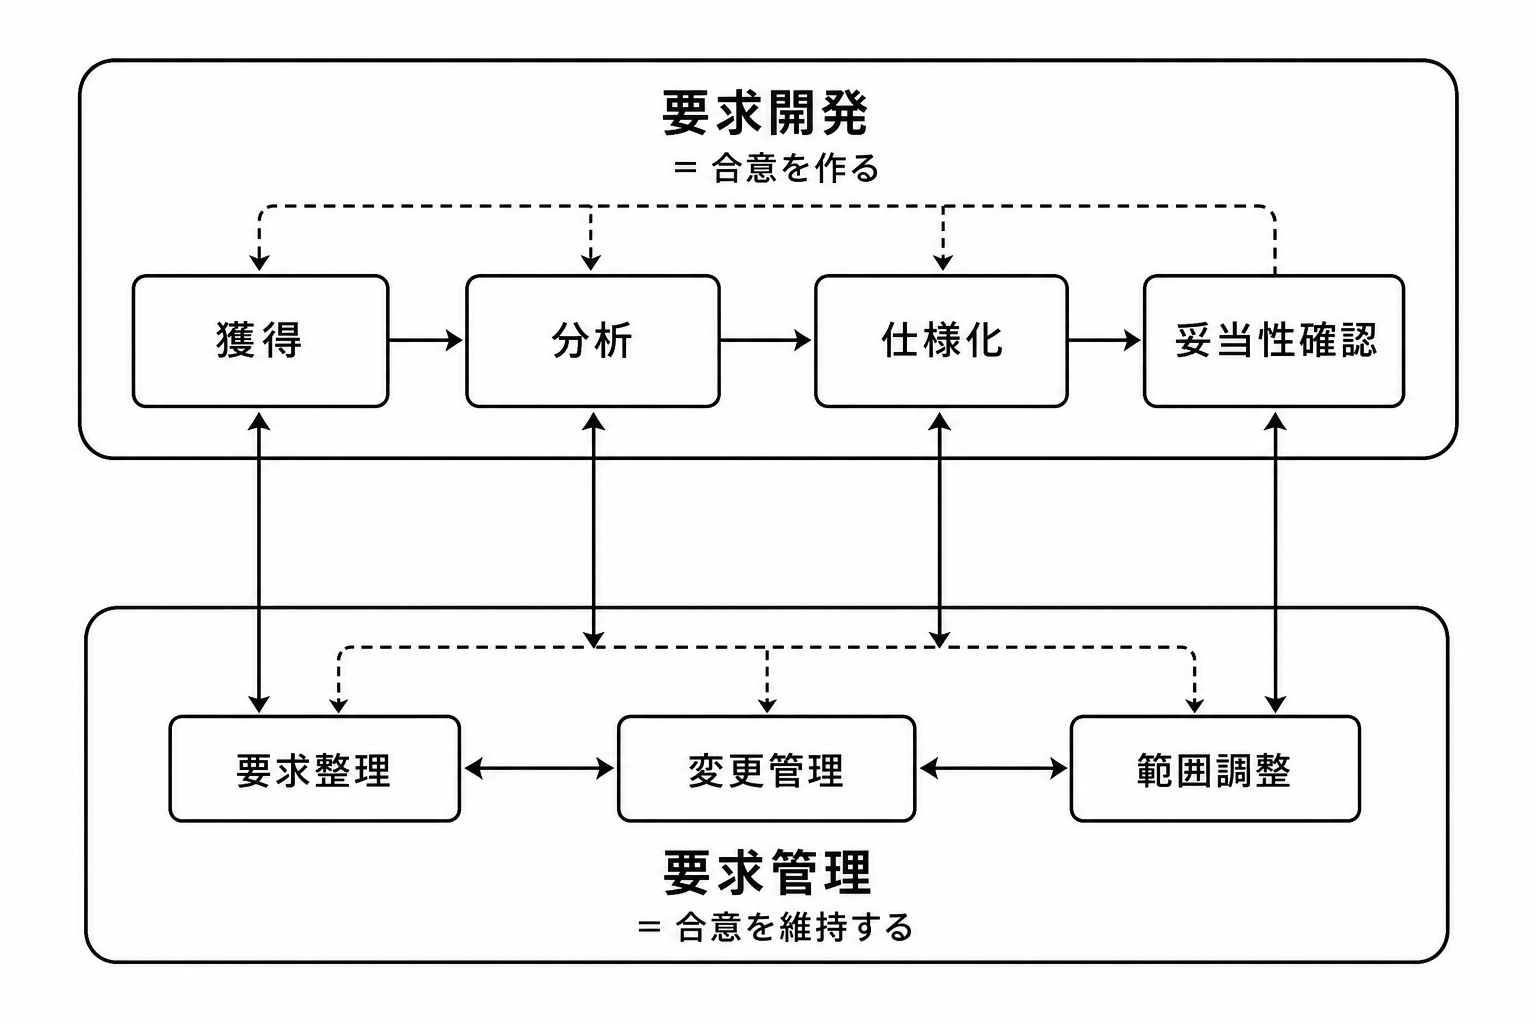
\includegraphics[width=0.96\linewidth]{assets/generated_figures/ch01/fig-ch01-05.png}}{\fbox{\parbox[c][48mm][c]{0.9\linewidth}{\centering 画像生成待ち\\要求開発と要求管理の活動図}}}
\caption{要求開発と要求管理の活動図}
\label{fig:ch01-05}
\end{figure}
